\beginsong{Au clair de la lune}
\beginverse*
Au clair de la lune, mon ami Pierrot. Prete-moi ta plume pour ecrire un mot. Ma chandelle est morte, je n'ai plus de feu, ourvre-moi ta porte pour l'amour de Dieu!
\endverse
\beginverse*
Au clair de la lune,Pierrot repondit: "Je n'ai pas de plume, Je suis dans mon lit. Va chez la voisine, Je crois qu'ell y est, car dans sa cuisine on bat le briquet."
\endverse
\beginverse*
Au clair de la lune, L'aimable Lubin. Frappe chew la brune, Ell' repond soudain: "Qui frappe d'la sorte?" Il dit a son tour: "Ouvrez votre porte pour le dieu d'amour!"
\endverse
\beginverse*
Au clair de la lune, On n'y voit qu'un peu. On chercha la plume, On chercha du feu. En chercant d'la sort, Je n'sais c' qu'on trouva: Mais j'sais que la porte  sur eux se ferma.
\endverse
\endsong
\begin{intersong}
    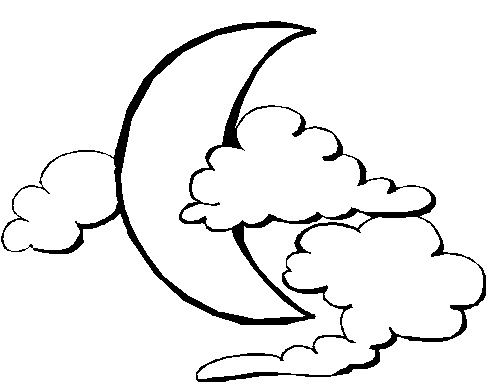
\includegraphics[width=0.4\textwidth]{img5}
\end{intersong}